\chapter{Aplicaciones de Mensajería}

Me voy a centrar en Telegram, Whatsapp y Facebook Chat, Signal y la de apple.

\section{Telegram (MTProto)}

Referencias: \cite{Miculan2021} \cite{WebProto}

\subsection{Descripción general}
MTProto 2.0 es una suite de protocolos criptográficos diseñados para implementar de manera rápida, escalable y segura intercambio de mensajes sin depositar esa responsabilidad en la seguridad del transporte debajo de dicho protocolo.
El protocolo esta subdividido en tres componentes virtuales independientes:
\begin{itemize}
	\item \textbf{Componente de alto nivel:} Define el método por el cual las consultas de la API y las respuestas se convierten en mensajes binarios. 
	\item \textbf{Capa criptográfica(autorización):} Define el método por el cual los mensajes están cifrados antes de ser enviados a través del protocolo de transporte.
	\item \textbf{Componente de transporte:} Define el método por el cual el cliente y el servidor para transmitir los mensajes sobre otro protocolo de red como HTTP, HTTPS, WS, WSS, TCP o UDP.
\end{itemize}

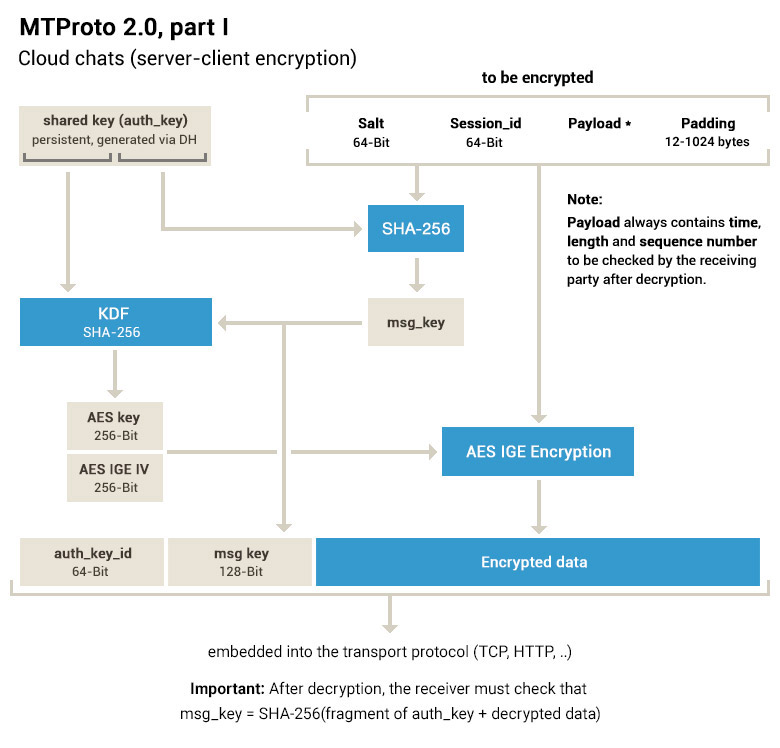
\includegraphics[scale=0.4]{imagenes/diagramaMTProto.jpg} 

\subsection{Resumen de los componentes}
\begin{description}
	\item \textbf{Componentes de alto nivel(Lenguajes de consulta/API RPC):}
Desde el punto de vista del componente de alto nivel, el cliente y el servidor intercambian mensajes dentro de una sesión.\\
La sesión se adjunta al cliente en lugar de una conexión \emph{websocket/http/https/tcp.} 
Además, cada sesión tiene asociada a clave ID de usuario mediante la cual se logra la autorización.\\ 
Pueden estar abiertas varias conexiones a un servidor, los mensajes pueden ser enviados en cualquier dirección a través de cualquiera de las conexiones.
Cuando se usa el protocolo UDP, una respuesta puede ser devuelta por una dirección de IP distinta.\\
Hay diferentes tipos de mensajes:
\begin{itemize}
		\item \textbf{LLamadas RPC(cliente-servidor):} LLamadas a los métodos de la API.
		\item \textbf{Respuestas RPC(servidor-cliente):} Resultados de las llamadas RPC.
		\item \textbf{Notificación del estado de los mensajes}
		\item \textbf{Consultas de estado de mensaje}
		\item \textbf{Mensaje multiparte o contenedor}
\end{itemize}
Desde el punto de vista de protocolos de bajo nivel, un mensaje es un flujo de datos alineados con 4 o 16 bytes de límite.
Los primeros campos en un mensaje están fijos y son usados por el sistema criptográfico o de autorización.\\
Cada mensaje, consiste en un \emph{Message Identifier} de 64 bits, \emph{número de secuencia del mensaje dentro de una sesión}, \emph{longitud} de 32 bits y \emph{cuerpo del mensaje} de cualquier tamaño siempre y cuando sea múltiplo de 4. 
Además cuando un contenedor o un mensaje simple se envían, una \emph{cabecera interna} se añade al principio del mensaje, luego el mensaje es cifrado y se le añade una \emph{cabecera externa} la cual será una \emph{clave de identificación} de 64 bits y una \emph{clave del mensaje} de 128 bits.\\
El \emph{cuerpo} del mensaje normalmente consiste en un \emph{tipo mensaje} de 32 bits seguido de los \emph{parámetros dependientes del tipo}.\\
Los números están escritos en \emph{little endian}. Sin embargo los números muy grandes(2048 bits) usados en \textbf{RSA} y \textbf{DH} están escritos en \emph{big endian} porque es lo que hace la biblioteca \textbf{OpenSSL}.
	\item \textbf{Autorización y Cifrado:}
			Antes de que un mensaje sea transmitido por la red usando un protocolo de transporte, este es cifrado añadiendo una cabecera externa la cual es insertada al principio del mensaje y contiene:
	\begin{itemize}
		\item \emph{Key Identifier} de 64 bits
		\item \emph{Message Key} de 128 bits
	\end{itemize}
Una clave de usuario junto con una clave de mensaje definen una clave de 256 bits la cual es la que cifra el mensaje usando un cifrado \emph{AES-256}.
La primera parte del mensaje cifrado contiene datos variables(sesión, id del mensaje, número de secuencia) los cuales influyen en la clave del mensaje. La clave del mensaje es definida como los 128 bits iniciales del mensaje cifrado con \emph{SHA-256}, 
además los mensajes en varias partes están cifrados como un solo mensaje.\\
Lo primero que tiene que hacer la aplicación cliente es crear una clave de autorización que se genera normalmente la primera vez que se ejecuta la aplicación y por lo general nunca cambia.\\
Para prevenir potenciales ataques debido a la apropiación de la clave de autorización MTProto soporta \emph{Perfect Forward Secrecy} tanto en los chats en la nube como en los chats secretos.
	\item \textbf{Sincronización de la hora:}
Si la hora de un cliente difiere de la hora del servidor, el servidor podría empezar a ignorar los mensajes de este y recíprocamente el cliente a los mensajes del servidor debido a que el mensaje tenga un indentificador inválido del mensaje.\\
Bajo estas circunstancias, el servidor enviará un mensaje especial al cliente el cual contendrá la hora correcta, este mensaje será el primero en el caso de que también se envíe un grupo de mensajes.\\
Habiendo recibido el mensaje, el cliente primero ejecutará una sincronización de la hora y después verificará la \emph{Message Key} para ver si es correcto.\\
En caso de que no sea correcto, el cliente deberá generar una nueva sesión para asegurar la monotonía de los \emph{Message Keys}.
\end{description}
\subsection{Modelo de seguridad}
Los protocolos de Telegram se modelan en ProVerif \cite{ProVer}, que es un verificador criptográfico simbólico. Los protocolos y propiedades de seguridad están especificadas en una variante del \emph{$\pi$-cálculo} que es una notación desarrollada por Robin Milner, Joachim Parrow y David Walker, como un avance sobre el cálculo de sistemas comunicantes con el fin de proveer movilidad al modelado concurrente para representar procesos criptográficos y traducirlos en una teoría de Horn.\\
MTProto 2.0 sigue la siguiente regla de reducción

\lstinputlisting[
    caption=Regla Reducción 1,
    label={lst:listing-cpp},
    language=C++,
    style=CodigoC,
    ]{./ejemplos/ejemplo1.cpp}

\subsection{Funcionamiento del protocolo}
La descripción del funcionamiento del protocolo la he obtenido de \cite{telegram2}. Previamente a explicar el funcionamiento de MTProto 2.0 voy a introducir las definiciones de los elementos más importantes que entrarán en juego durante el funcionamiento de este.\\
\begin{description}
	\item \textbf{Authorization Key (auth\textunderscore key)}\\
	Es una clave de 2048 bit compartida por el dispositivo del cliente y el servidor, se crea durante el registro del usuario, se almacena en el dispositivo de este mediante el protocolo de intercambio de claves \emph{Diffie-Hellman} y nunca se transmite a través de la red. Cada clave de autorización es única y dependiente del usuario, aunque un usuario puede tener más de una ya que Telegram permite tener sesiones persistentes en diferentes dispositivos. En caso de ser necesario estas claves pueden ser bloqueadas para siempre como por ejemplo podría pasar si un dispositivo con sesión persistente se pierde.

	\item \textbf{Server Key}\\
	Es una clave RSA de 2048 bits usada por el servidor para firmar sus mensajes durante el proceso de registro y la clave se está generando. La aplicación tiene una clave publica del servidor que puede ser utilizada para verificar la firmas pero no para firmar mensajes. La clave privada del servidor es almacenada en este y raramente cambia.

	\item \textbf{Key Identifier (auth\textunderscore key\textunderscore id)}\\
	Se usan los 64 bits menos significativos del hash \emph{SHA1} de la \emph{Authorization Key} para indicar que clave en particular se ha usado para cifrar el mensaje. Las claves tienen que ser identificadas unívocamente y en caso de colisión, la \emph{Authorization Key} se regenera. Un identificador Zero Key significa que el cifrado no se usa y esto está permitido para muy pocos mensajes usados durante el registro para generar la clave en el intercambio \emph{Diffie-Hellman}.
	
	\item \textbf{Session}\\
	Es un número de 64 bits generado aleatoriamente por el cliente para distinguir entre sesiones individuales como pueden ser diferentes instancias de la aplicación creadas con la misma \emph{Authorization Key} donde una instancia de la aplicación es la conjunción de la \emph{Key Identifier} y la \emph{Session}.\\
	Bajo ninguna circunstancia un mensaje perteneciente a una sesión puede ser enviado a otra.

	\item  \textbf{Server Salt}\\
	Es un número de 64 bits generado aleatoriamente que cambia cada 30 minutos independiente de las sesiones por una petición del servidor. Una vez generado el nuevo salt todos los mensajes tienen que tenerlo aunque se aceptan los mensajes con el salt previo. Es necesario para proteger ante ciertos ataques como podría ser ajustar el reloj de la víctima en un momento futuro.

	\item \textbf{Message Identifier (msg\textunderscore id)}\\
	Es un número de 64 bits dependiente del tiempo usado únicamente para identificar mensajes sin sesión. Los \emph{Message Identifiers} son divisibles por 4, los \emph{Message Identifiers} del servidor módulo 4 dan 1 si el mensaje es una respuesta a un mensaje del cliente y dan 3 en otro caso. 
	Los \emph{Message Identifiers} del cliente deben incrementarse monótonamente, igualmente con los del servidor y tienen que ser aproximadamente igual a $unixtime*2^{32}$, donde \emph{unixtime} es un sistema para la descripción de instantes de tiempo definida como la cantidad de segundos transcurridos desde la medianoche UTC del 1 de enero de 1970. 
	De esta manera, el \emph{Message Identifier} señala el momento aproximado en el que el mensaje fue creado siendo rechazado alrededor de 300 segundos después o 30 segundos antes de ser creado (necesario como medida de protección de ataques de repetición).  

	\item \textbf{Content-related Message}\\
	Un mensaje requiere un reconocimiento explícito. Esto incluye todos los mensajes de usuario y muchos de servicio, a excepción de contenedores y otros reconocimientos.

	\item \textbf{Message Sequence Number (msg\textunderscore seqno)}\\
	Un número de 32 bit igual o el doble del número de mensajes \emph{content-related} creados por el remitente antes de este mensaje y posteriormente se va incrementado en uno si el mensaje es del tipo \emph{cotent-related}. Cabe a destacar que como un contenedor se genera después de su contenido, su \emph{Message Sequence Number} será siempre igual o mayor a los números de mensajes contenidos en él.

	\item \textbf{Message Key (msg\textunderscore key)}\\
	En el protocolo \textbf{MTProto 2.0}, la \emph{Message Key} se define como los 128 bits del medio del hash \emph{SHA-256} del mensaje que va a ser cifrado antepuesto por un fragmento de 32 bytes de la clave de autorización.\\
	En el protocolo \textbf{MTProto 1.0}, la \emph{Message Key} se definía como los 128 bits menos significativos del hash \emph{SHA-1} del mensaje a ser cifrado, los bytes de relleno eran excluidos en el cálculo del hash. La \emph{Authorization Key} no estaba involucrada en este cálculo.

	\item \textbf{Internal (cryptographic) Header}\\
	Una cabecera de 16 bytes añadida antes de que el mensaje o el contenedor sea cifrado. Consiste en el \emph{Server Salt} de 64 bits y la \emph{Session} de 64 bits.

	\item \textbf{External (cryptographic) Header}\\
	Una cabecera de 24 bytes que se añade antes de que el mensaje o el contenedor sea cifrado. Consiste en la \emph{auth\textunderscore key\textunderscore id} de 64 bits y la \emph{msg\textunderscore key} de 128 bits.

	\item \textbf{Payload}\\
	Es el \emph{External Header} + mensaje cifrado o contenedor.
\end{description}
